\section{Proyecto principal}
%
%
Este trabajo trataba de la optimización del gasto energético de una empresa que contaba con hornos de fundición. Para ello, se tuvieron que realizar predicciones del precio de la electricidad mediante modelos estadísticos. Posteriormente, se modelizó el proceso de fundición llevado a cabo en la fábrica y por último se trató de optimizar la selección de los materiales a fundir, dependiendo del espacio disponible en fábrica y el precio de la luz en cada tramo horario, estimado previamente.
%
%
\subsection{Predicción de precios de la luz}
%
%
%
%
Para llevar a cabo un modelo predictivo de los precios de la luz para una empresa hemos de realizar una serie de pasos. En primer lugar, como es evidente, debemos conocer y entender qué es lo que queremos predecir, bajo qué condiciones y qué variables afectan al precio de la luz, tanto naturales, como puede ser la demanda, la generación de ciertos tipos de energía, como aquellas relacionadas con la legislación vigente. Posteriormente debemos decidir cómo se extraeran los datos necesarios. Puesto que estamos hablando de un proyecto real, la empresa espera un proceso automatizado por lo que se debe tener en cuenta una extracción periódica de datos.

Una vez planteado el contexto en el que vamos a movernos, debemos decidir qué modelos probar, conociendo sus ventajas y desventajas. Mi elección, basada en búsquedas de desarrollos similares, fue optar por tres modelos:
\begin{description}
    \item[SARIMAX:] Modelo estadístico clásico.
    \item[Random Forest:] Modelo de \textit{machine learning} basado en árboles de decisión.
    \item[XGBoost:] Modelo de \textit{machine learning} basado en árboles de decisión, más avanzado que el anterior.
    \item[TFT:] Modelo de \textit{deep learning}, específico para series temporales.
\end{description}

Por último, por requisitos del proyecto, la predicción se realizaba a un mes vista, lo cual como es lógico, no es óptimo. Sin embargo, esto era algo fijo por lo que los resultados esperados son mejorables, recortando el horizonte de predicción y reentrenado los modelos con mayor asiduidad.
%
%
%
\subsubsection{Estudio y comprensión del mercado}
%
%
%
Dado que la empresa es una electrointensiva no se rige por el régimen general del pequeño consumidor (PVPC). Para la toma de datos de la variable objetivo, el precio de la luz, se consultó el precio del mercado SPOT diario, que es el que regula la venta de luz al por mayor.

Para calcular exactamente, dentro de lo que podemos entender como \textit{exacto} en un modelo de predicción, el precio de la luz debemos tener en cuenta tanto el precio de venta como los peajes. Estos últimos son valor añadido a la factura de la luz que depende del tipo de empresa y de la hora de consumo. De cualquier forma, en lo que a nuestro modelo se refiere, únicamente nos interesa el precio del mercado SPOT diario, que viene dado de manera horaria.
%
%
%
\subsubsection{Obtención y preparación de los datos}
%
%
%
Los datos se obtuvieron a través de la API pública proporcionada por ESIOS (Sistema de Información del Operador del Sistema Eléctrico), que permite acceder a los precios horarios históricos, así como a otros indicadores del sistema eléctrico. De manera adicional al precio de la luz, y como se ha comentado previamente, se tomaron variables explicativas, es decir, que se cree que tienen relación y afectan al precio de la que queremos. En este caso, se tomó: La demanda real de consumo, la generación de energía eólica y solar.

En lo relativo a la preparación de los datos, salvando las diferencias en función de la implementación del modelo, el procedimiento fue similar: Una vez descargados los datos se formatean de manera que tengamos aquellos valores que queremos, es decir, el precio, demanda, etc. y la fecha en la que se dio. Además, para refinar nuestro modelo, se introdujeron variables temporales como el día de la semana, día del mes o mes del año. Un estudio mucho más exhaustivo puede hacerse incluyendo más variables o con más combinaciones. En \cite{TFG_prediccion} puede verse cómo incluyen el precio del gas o la emisión de CO$_2$ entre otros, llevándoles a mejores resultados, aunque con mayor trabajo.
%
%
%
\subsubsection{Análisis exploratorio}
%
%
%
Este proceso consiste en la observación de los datos, su representación en diferentes formas con el fin de decidir características del modelo. El estudio consistió en graficar respecto del tiempo el histórico de datos, implementar una matriz de correlación para observar las relaciones entre las distintas variables y boxplot para estudiar el comportamiento de nuestra serie.

A partir de los datos obtenidos con las gráficas, como se puede observar en la figura \cref{Precio vs tiempo}, se divide el histórico de datos en un conjunto de entrenamiento, otro de test y se deja uno de validación, en este caso de un mes, al igual que la predicción que queremos realizar, para comprobar el funcionamiento \textit{real} de nuestro modelo. Este proceso es el que se ha utilizado en la SARIMAX, Random Forest y el XGBoost.

Observando la matriz de correlación (\cref{Matriz de correlacion}) se aprecia que la variable con mayor correlación negativa con el precio es la generación solar ($r \approx -0.38$), lo que sugiere que un aumento en la producción solar tiende a asociarse con una disminución en el precio. La demanda real presenta una correlación positiva moderada ($r \approx 0.25$) con el precio, mientras que la generación eólica muestra una relación más débil y ligeramente negativa. Las variables temporales (hora, día de la semana, mes) tienen correlaciones bajas, lo que indica que, si bien influyen en el precio, lo hacen de forma más indirecta o no lineal.

En cuanto a los boxplots, puede observarse cómo en el ámbito anual (figura \cref{Boxplotanual}) los meses de abril y mayo concentran los precios más bajos, mientras que en febrero se registran picos más altos. También se aprecia que la variabilidad del precio es mayor en los meses de invierno y menor en primavera. En el análisis diario (figura \cref{Booxplotdiario}), se identifican claramente las denominadas \textit{horas valle}, comprendidas aproximadamente entre las 10:00 y las 15:00, y las \textit{horas pico}, situadas en el tramo de 18:00 a 20:00. 

\begin{figure}[H]
\centering
\begin{subfigure}[b]{0.7\textwidth}
\centering
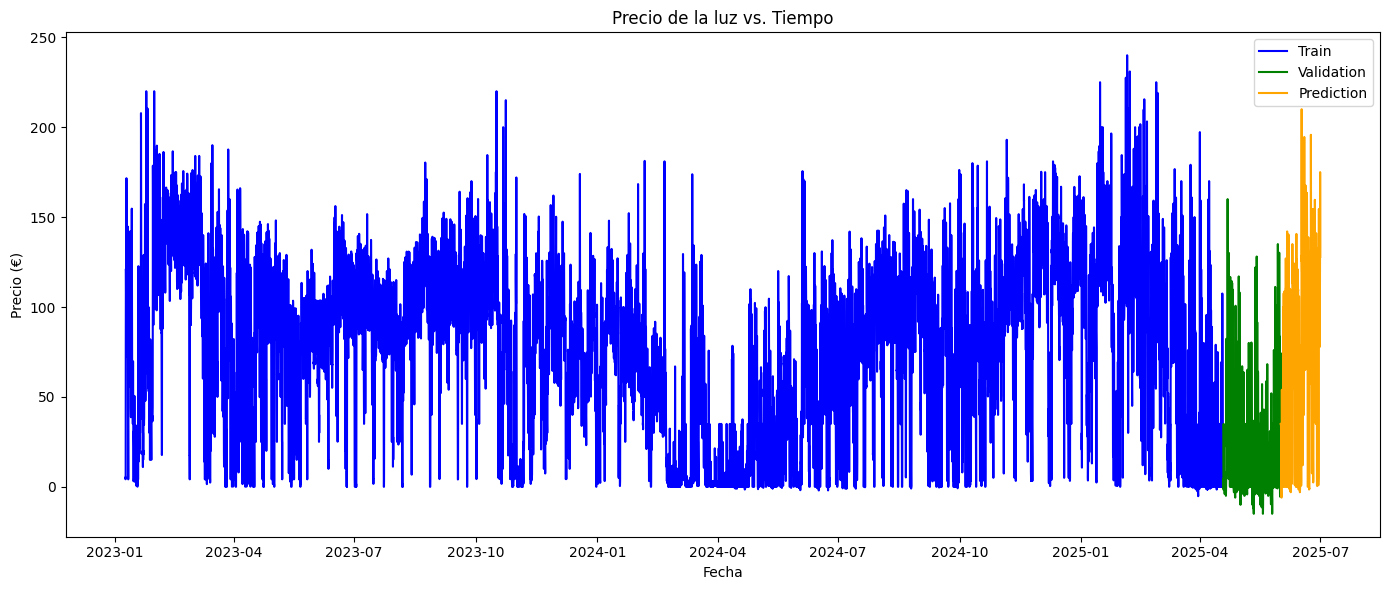
\includegraphics[width=\textwidth]{figuras/historico_precios.png}
\caption[Precio de la luz respecto del tiempo]{Precio de la luz respecto del tiempo, en azul se ve el conjunto de entrenamiento (\textit{train test}), en verde el conjunto de test (\textit{test test}) y en amarillo el conjunto de validación (\textit{validation test}).}
\label{Precio vs tiempo}
\end{subfigure}
\begin{subfigure}[b]{0.6\textwidth}
\centering
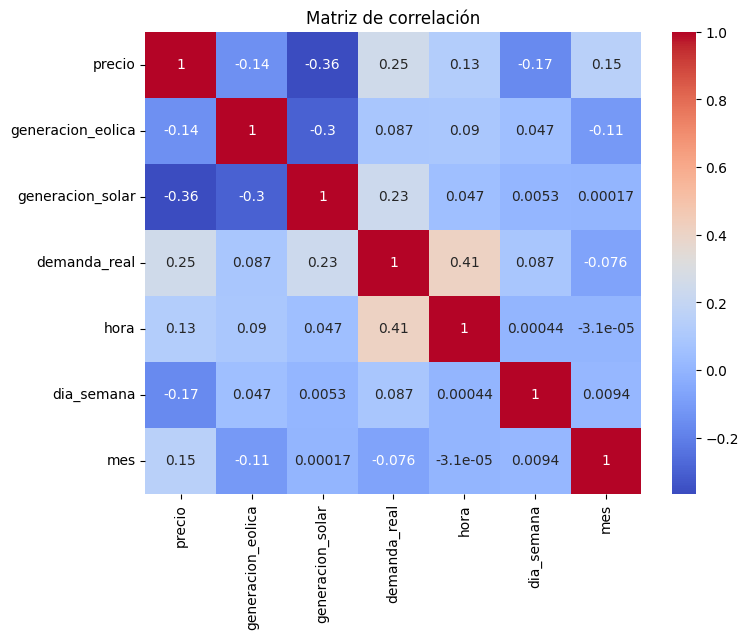
\includegraphics[width=\textwidth]{figuras/matriz_correlacion.png}
\caption[Matriz de correlación]{Matriz de correlación.}
\label{Matriz de correlacion}
\end{subfigure}
\begin{subfigure}[b]{0.4\textwidth}
\centering
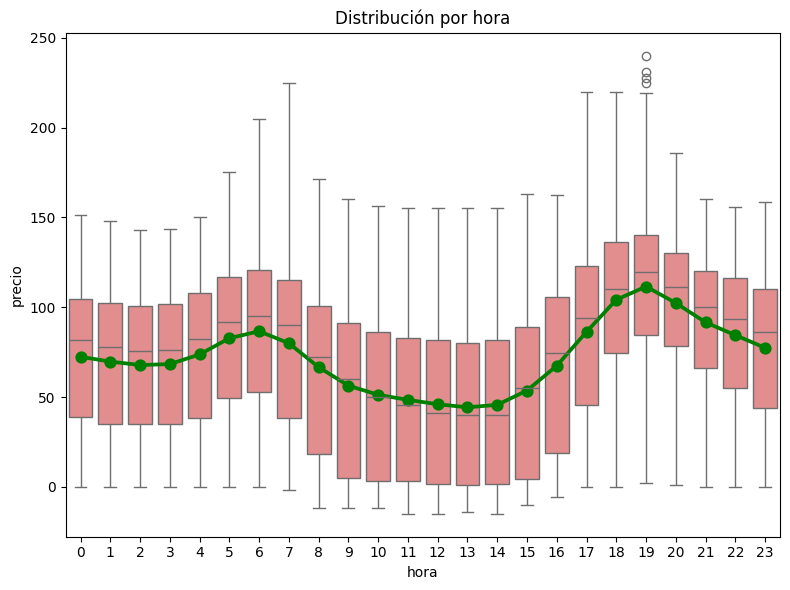
\includegraphics[width=\textwidth]{figuras/boxplot_diario.png}
\caption[Boxplot diario]{Boxplot diario.}
\label{Booxplotdiario}
\end{subfigure}
\begin{subfigure}[b]{0.4\textwidth}
\centering
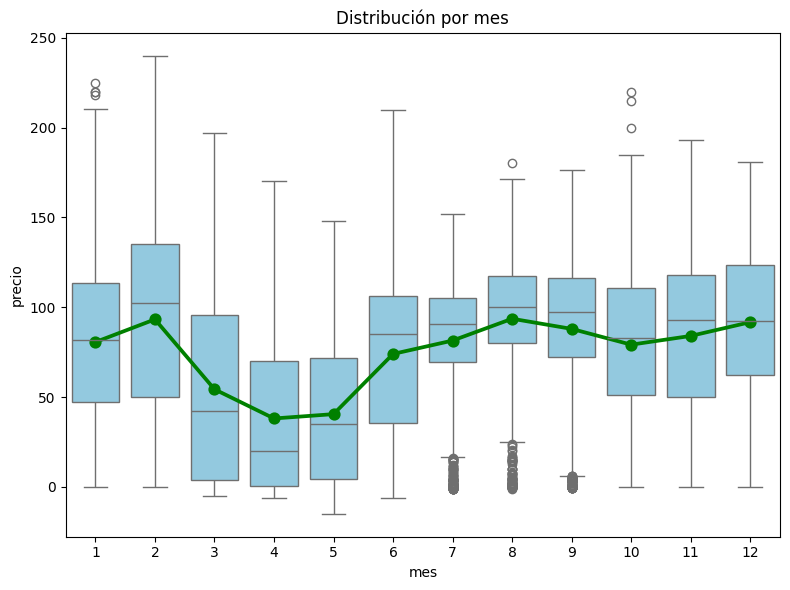
\includegraphics[width=\textwidth]{figuras/boxplot_anual.png}
\caption[Boxplot anual]{Boxplot anual.}
\label{Boxplotanual}
\end{subfigure}
\caption{Figuras del análisis exploratorio.}
\label{Análisis exploratorio}
\end{figure}
%
%
%
\subsubsection{SARIMAX}
%
%
%
Este es un modelo estadístico clásico para la predicción de series temporales. Su fortaleza radica en su capacidad para modelar explícitamente tres componentes clave de la serie:

\begin{itemize}
    \item \textbf{Tendencia (I - Integrado):} Se logra a través de la diferenciación para hacer que la serie sea estacionaria.
    \item \textbf{Estacionalidad (S - Seasonal):} Captura patrones que se repiten en intervalos fijos (por ejemplo, diarios o semanales).
    \item \textbf{Variables (X):} Permite incluir predictores externos, como la demanda o la generación de energía.
\end{itemize}

El proceso consiste en:
\begin{itemize}
    \item \textbf{Identificación:} El modelo SARIMAX viene caracterizado por los valores $(p,d,q)x(P,D,Q,s)$ donde:
        \begin{itemize}
        \item[$p:$] Orden del componente autorregresivo (AR) no estacional. Indica el número de rezagos de la variable endógena que se incluyen en el modelo.
        \item[$d:$] Orden de diferenciación no estacional. Representa la cantidad de veces que se deben diferenciar los datos para hacer la serie estacionaria.
        \item[$q:$] Orden del componente de media móvil (MA) no estacional. Indica el número de rezagos del error del pronóstico que se incluyen en el modelo.
        \item[$P:$] Orden del componente autorregresivo (AR) estacional.
        \item[$D:$] Orden de diferenciación estacional.
        \item[$Q:$] Orden del componente de media móvil (MA) estacional.
        \item[$s:$] Período de estacionalidad, en este caso vemos que $s=24$ de manera natural al tratarse de precios horarios.
    \end{itemize}
    
    \item \textbf{Estimación:} Una vez definidos los órdenes, se ajusta el modelo al conjunto de datos de entrenamiento. El modelo aprende los coeficientes que ponderan la importancia de los valores pasados, los errores de pronóstico pasados y las variables exógenas.
\end{itemize}

La predicción con SARIMAX es un proceso iterativo o recursivo:
\begin{itemize}
    \item \textbf{Entrenamiento:} Al igual que con otros modelos, se reentrena un modelo SARIMAX final con su orden óptimo utilizando todos los datos históricos disponibles para maximizar la información aprendida.
    
    \item \textbf{Predicción:} Para predecir el horizonte futuro (ej. las próximas 24 horas), el modelo:
    \begin{itemize}
        \item Predice el primer paso $(t+1)$ utilizando todos los datos históricos reales.
        \item Para predecir el segundo paso $(t+2)$, utiliza los datos históricos y la predicción que acaba de hacer para t+1 como si fuera un dato real.
    \end{itemize}
\end{itemize}

Este proceso se repite para cada punto en el horizonte de predicción.

En nuestro caso, para determinar los órdenes de los hiperparámetros del modelo, se analizan las funciones de autocorrelación (ACF) y autocorrelación parcial (PACF). La ACF mide la correlación de la serie consigo misma en diferentes rezagos, mientras que la PACF mide esta misma correlación eliminando la influencia de los rezagos intermedios.

En las siguientes imágenes podemos ver los gráficos de ACF y PACF para la serie de precios de la luz, lo que nos permite identificar los patrones de estacionalidad y los órdenes de los modelos.

\begin{figure}[H]
    \centering
    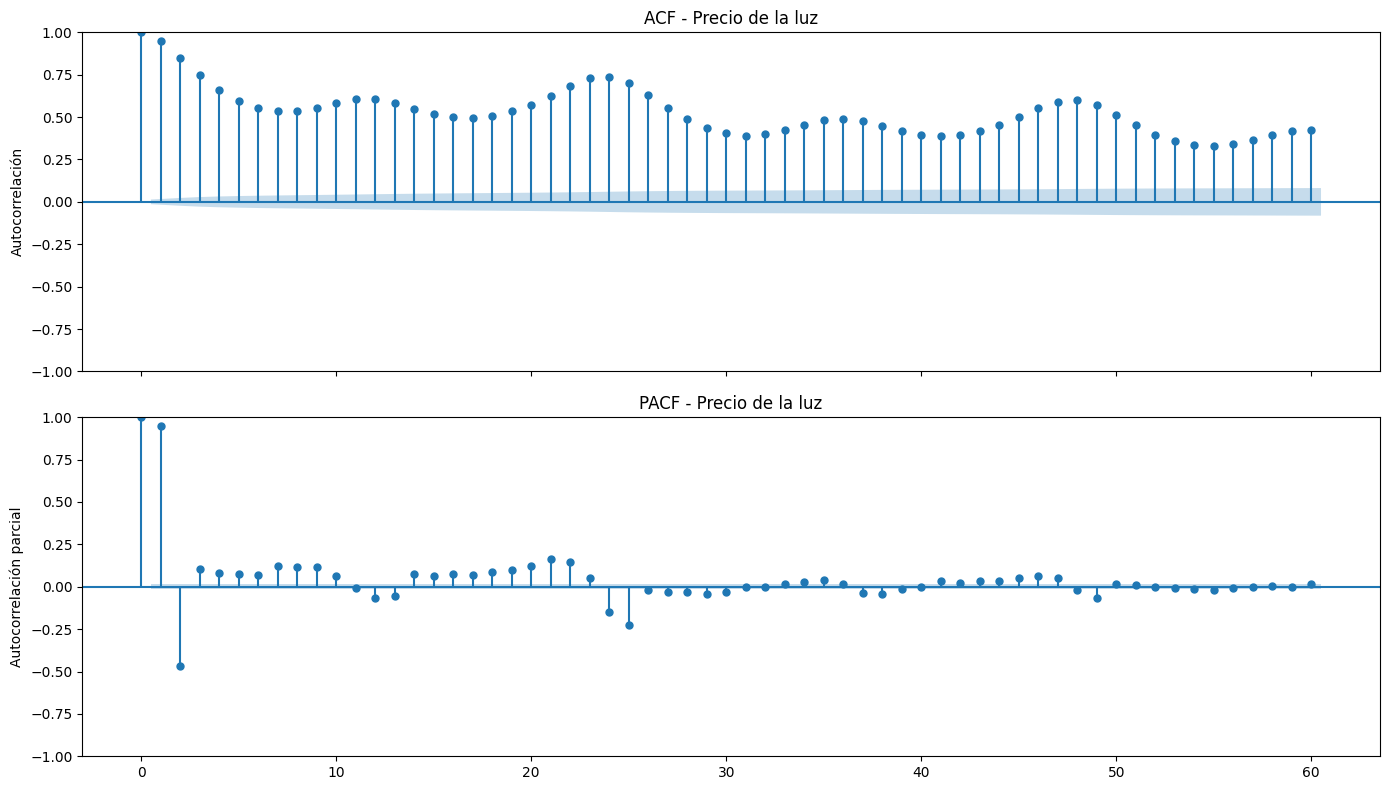
\includegraphics[width=0.7\linewidth]{figuras/ACFPACFdD0.png}
    \caption[ACF y PACF serie temporal original.]{Podemos observar el ACF y el PACF de la serie temporal original, sin diferenciación. En ellos podemos ver que hay una clara estacionalidad alrededor del lag 24, lo que concuerda con el pensamiento de una periodicidad diaria, cada 24 horas. Además, que no haya un decaimiento fuerte hace pensar que requiera diferenciación.}
    \label{ACFPACFDd0}
\end{figure}
\begin{figure}[H]
    \centering
    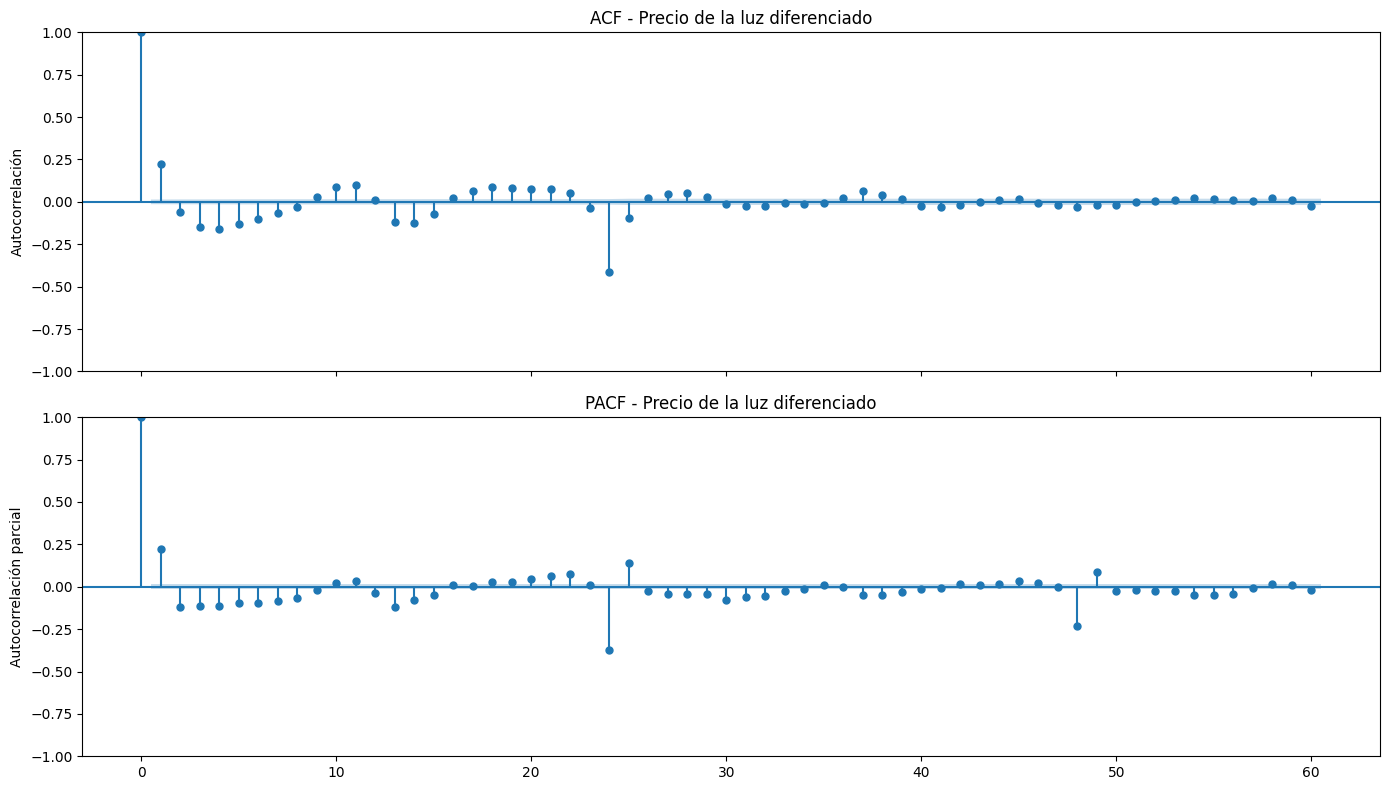
\includegraphics[width=0.7\linewidth]{figuras/ACFPACFdD1.png}
    \caption[ACF y PACF serie temporal diferenciada $d=D=1$.]{De nuevo, es visible la periodicidad en los picos con estacionalidad 24, sin embargo, esta vez se aprecia la caída en los picos, lo que sugiere haber encontrado ya la estacionariedad, además de que esto nos ayuda a determinar los posibles órdenes, como $p,P,Q,q \in \{0,1,2\} $.}
    \label{ACFPACFDd1}
\end{figure}

Basado en el análisis de las funciones de autocorrelación y en una herramienta, \textit{pmdarima}, que permite probar y obtener los órdenes óptimos, se han seleccionado los siguientes tres modelos, donde se muestran las gráficas de predicción obtenidas:

\begin{itemize}
    \item \textbf{Modelo 1: SARIMAX(2,1,1)x(1,1,1,24)}:
    \begin{figure}[H]
    \centering
    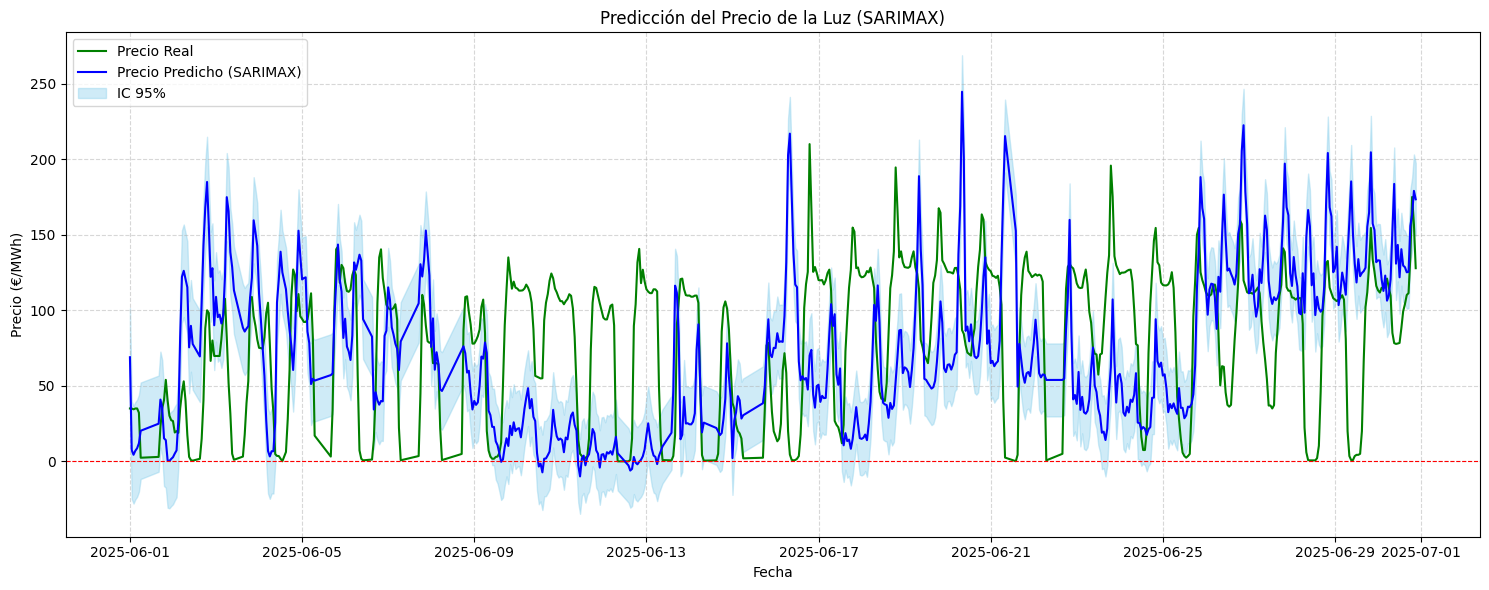
\includegraphics[width=0.60\linewidth]{figuras/SARIMAX_pred21011024.png}
    \caption[Predicción SARIMAX (2,1,1)x(1,1,1,24)]{Predicción para junio con el SARIMAX de órden (2,1,1)x(1,1,1,24).}
    \label{SARIMAX (2,1,1)x(1,1,1,24)}
    \end{figure}


    \item \textbf{Modelo 2: SARIMAX(1,1,1)x(1,1,1,24)}:
    \begin{figure}[H]
    \centering
    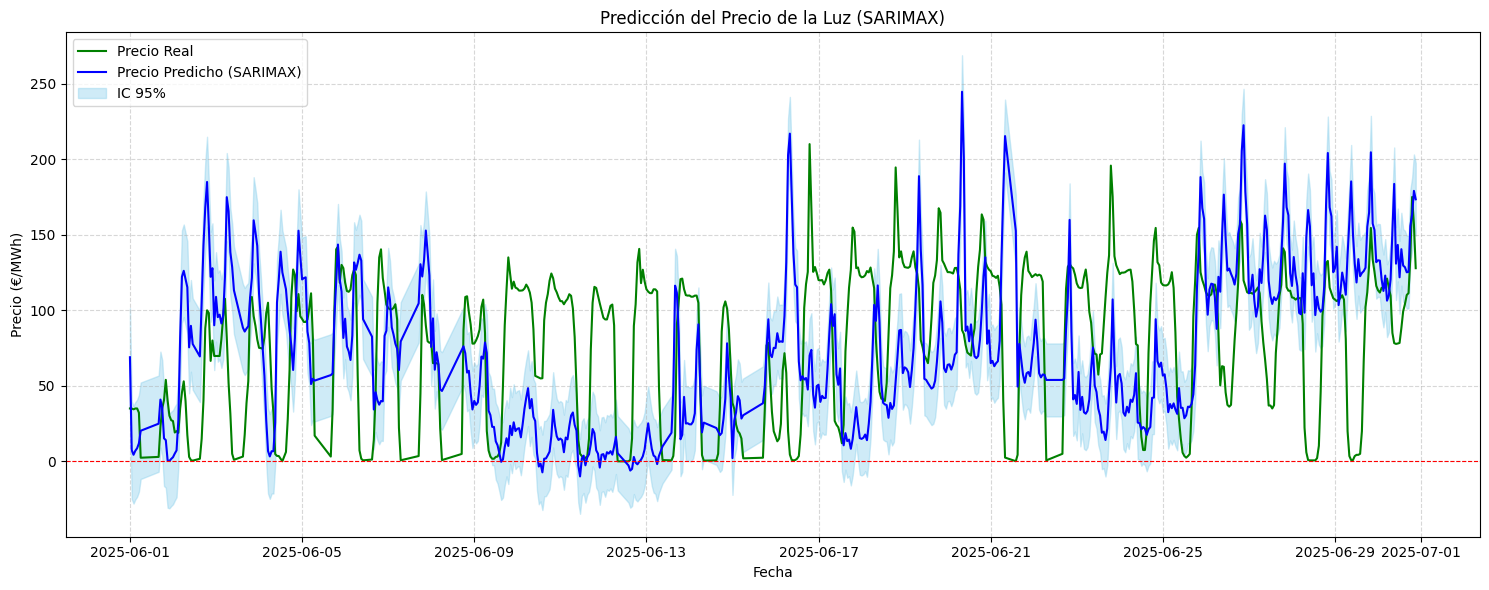
\includegraphics[width=0.60\linewidth]{figuras/SARIMAX_pred21011024.png}
    \caption[Predicción SARIMAX (1,1,1)x(1,1,1,24)]{Predicción para junio con el SARIMAX de órden (1,1,1)x(1,1,1,24).}
    \label{SARIMAX (1,1,1)x(1,1,1,24)}
    \end{figure}


    \item \textbf{Modelo 3: SARIMAX(2,1,0)x(1,1,0,24)}: 
    \begin{figure}[H]
    \centering
    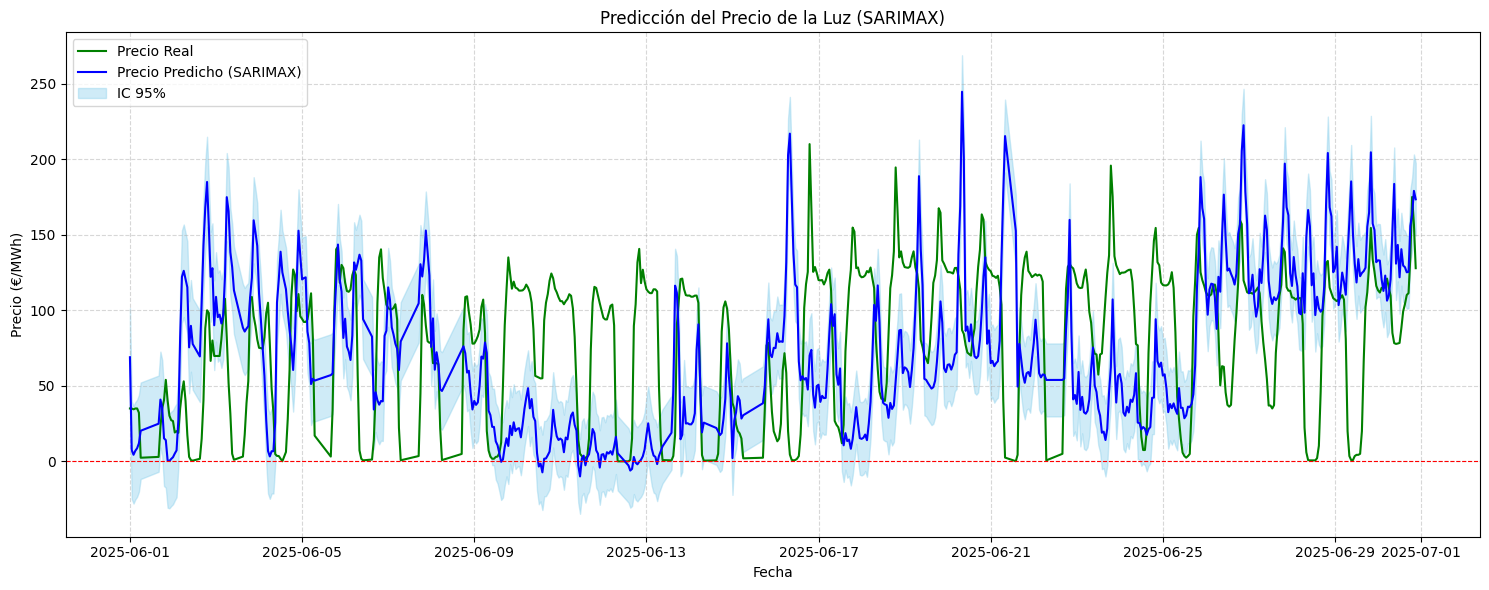
\includegraphics[width=0.60\linewidth]{figuras/SARIMAX_pred21011024.png}
    \caption[Predicción SARIMAX (2,1,0)x(1,1,0,24)]{Predicción para junio con el SARIMAX de órden (2,1,0)x(1,1,0,24).}
    \label{SARIMAX (2,1,0)x(1,1,0,24)}
    \end{figure}
    
 
\end{itemize}

Puede apreciarse a simple vista que para un horizonte de predicción de un mes este método no es fiable. El modelo SARIMAX supone relaciones lineales y la volatilidad y complejidad del precio de la luz, además en un intervalo de tiempo tan grande como un mes no reporta predicciones satisfactorias.
%
%
%
\subsubsection{Random Forest}
%
%
%
Este modelo, también basado en árboles de decisión, destaca por su sencillez de implementación y su gran versatilidad para distintos tipos de problemas, aunque, como ocurre habitualmente en modelos de este tipo, presenta una menor interpretabilidad sobre el funcionamiento interno. Su fortaleza radica en el uso de un enfoque de ensamblado (\textit{ensemble}) mediante \textit{bagging}, que combina múltiples árboles de decisión entrenados de manera independiente a partir de bootstrap y predictores. Este procedimiento permite reducir la varianza del modelo y mejorar la capacidad de generalización, incluso sin requerir un ajuste tan fino como otros métodos más complejos. Entre las características más relevantes de Random Forest:

\begin{itemize}
    \item \textbf{Robustez frente al \textit{overfitting}:} El uso de múltiples árboles entrenados con subconjuntos aleatorios ayuda a evitar que el modelo memorice el conjunto de entrenamiento, reduciendo el riesgo de sobreajuste.
    \item \textbf{Capacidad de manejo de datos ruidosos:} El promedio (en regresión) o el voto mayoritario (en clasificación) suaviza el impacto de observaciones atípicas.
    \item \textbf{Manejo de variables de distinta naturaleza:} Puede trabajar tanto con variables numéricas como categóricas sin necesidad de una normalización previa.
    \item \textbf{Importancia de variables:} Aunque la interpretación global es limitada, proporciona métricas de importancia relativa para cada predictor, lo que facilita la identificación de los más influyentes.
\end{itemize}

En nuestro caso, la implementación con la librería \textit{scikit-learn} permite optimizar el modelo mediante herramientas como \textit{TimeSeriesSplit} y \textit{GridSearchCV}, especialmente útiles en problemas de series temporales. De nuevo, nos enfrentamos a dos retos principales: la selección de hiperparámetros y la evaluación de errores.

Para la evaluación, \textit{TimeSeriesSplit} divide el conjunto de entrenamiento en particiones cronológicas, evitando la ruptura de la secuencia temporal y permitiendo calcular métricas como MAE, RMSE o R$^2$ de forma más realista.

En cuanto a la búsqueda de los hiperparámetros óptimos (\textit{hyperparameter tuning}), \textit{GridSearchCV} prueba combinaciones dentro de los rangos definidos y nos devuelve la configuración con mejor rendimiento según una métrica objetivo, como el RMSE. En las siguientes gráficas mostramos los resultados obtenidos en uno de los entrenamientos junto a sus errores:
\begin{figure}[H]
    \centering
    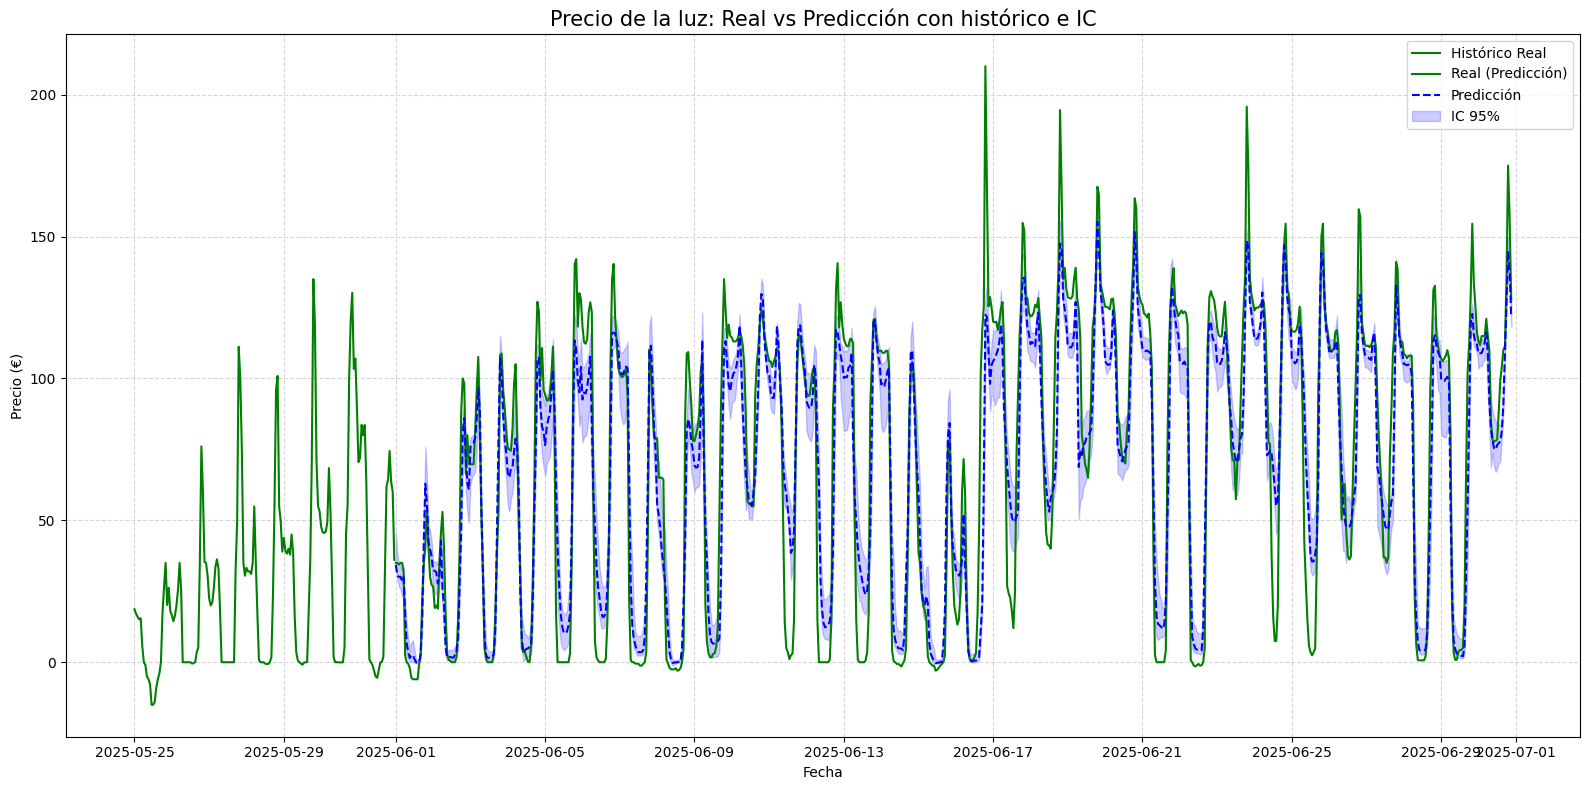
\includegraphics[width=0.7\linewidth]{figuras/RandomForest_prediccion.png}
    \caption[Predicción con Random Forest]{Predicción realizada para el mes de junio de 2025 con un entrenamiento sobre el histórico completo de datos.}
    \label{RandomForest_prediccion}
\end{figure}

\begin{figure}[H]
    \centering
    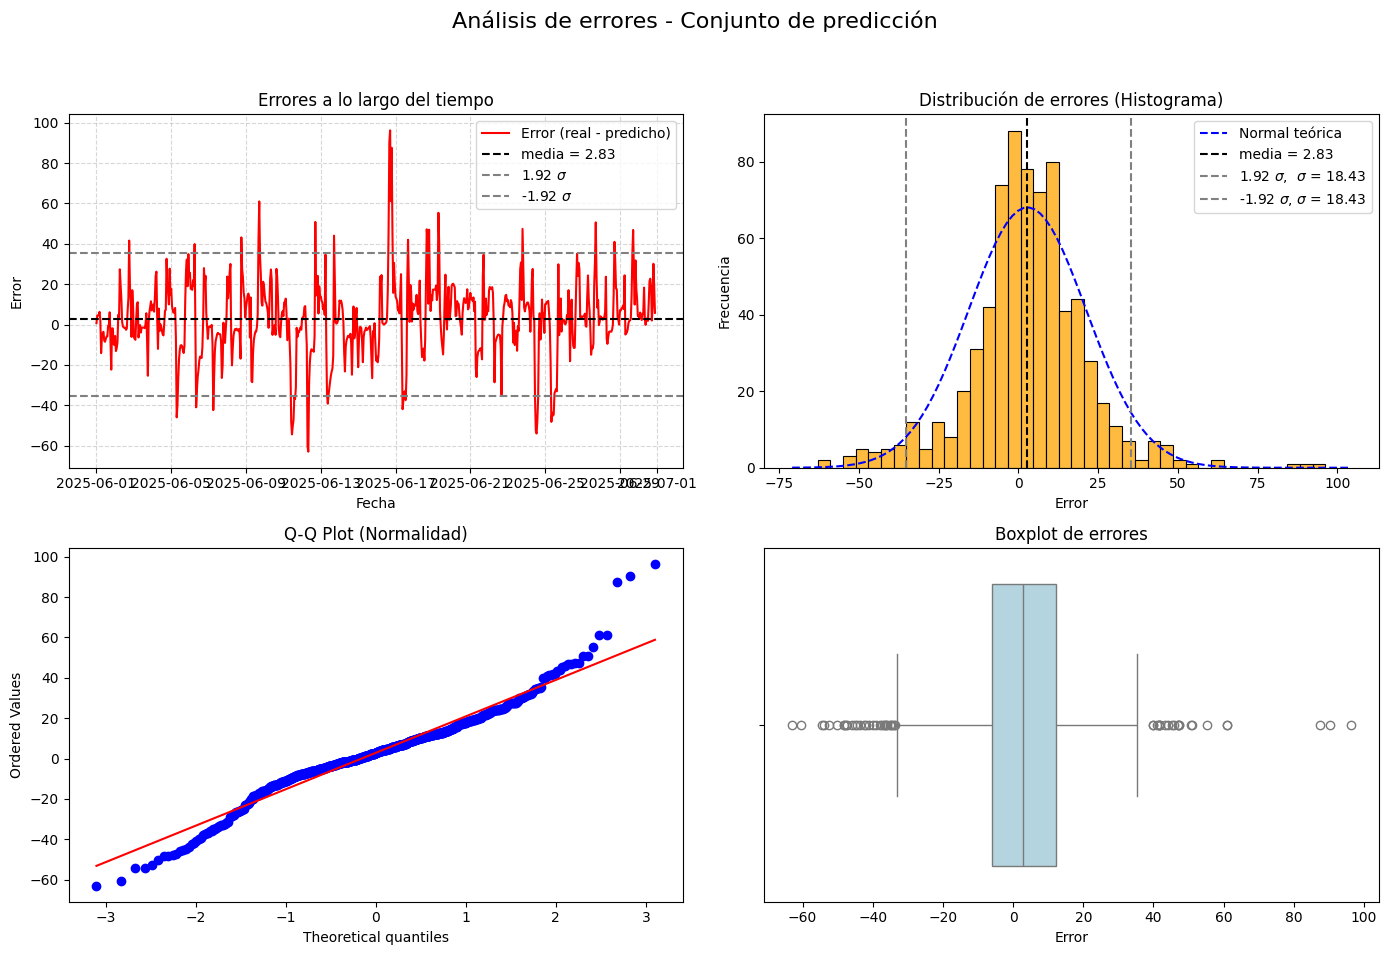
\includegraphics[width=0.7\linewidth]{figuras/RandomForest_errorespng.png}
    \caption[Errores en predicción con Random Forest]{Errores del modelo Random Forest, donde los QQ-plots y el histograma muestran una distribución simétrica, sin colas pesadas pero no completamente normal.}
    \label{RandomForest_errores}
\end{figure}
%
%
%
\subsubsection{XGBoost}
%
%
%
Este modelo, basado en árboles de decisión, también es relativamente sencillo de implementar aunque, como es habitual en este tipo de modelos, presenta menor interpretabilidad respecto a lo que ocurre dentro del algoritmo. Su robustez radica en la capacidad de aprender patrones complejos mediante un enfoque de ensamblado (\textit{ensemble}) y mejora por aproximación secuencial de errores. Además, se ve reforzado por técnicas de regularización y control del \textit{overfitting}, lo que permite obtener modelos generalizables y eficientes en predicción.Entre las características más destacadas de XGBoost:

\begin{itemize}
    \item \textbf{Regularización integrada:} A diferencia de otros modelos basados en árboles, XGBoost incluye regularización $L_1$ y $L_2$ como parte de la función de coste, permitiendo controlar la complejidad del modelo y reducir el riesgo de \textit{overfitting}.
    \item \textbf{Manejo de valores nulos:} Tiene un tratamiento nativo para valores faltantes, aprendiendo automáticamente la mejor dirección en los nodos de decisión.
    \item \textbf{Velocidad y eficiencia:} Permite la construcción de árboles de manera paralela. Además, utiliza una aproximación de segundo orden (Taylor) sobre la función de pérdida, incorporando tanto el gradiente como el hessiano. Esto no solo acelera la convergencia del modelo, sino que también permite trabajar con funciones de pérdida más generales, si bien lo más común es trabajar con el error cuadrático medio.
    \item \textbf{Importancia de variables:} Aunque la interpretabilidad del modelo global es limitada, permite extraer métricas de importancia relativa de cada predictor.
\end{itemize}

El entrenamiento se realiza mediante un enfoque de \textit{boosting}:

\begin{itemize}
    \item \textbf{Inicialización:} Se parte de una predicción base (por ejemplo, la media de la variable a predecir).
    \item \textbf{Aprendizaje secuencial:} Cada árbol posterior intenta corregir los errores residuales cometidos por el conjunto acumulado hasta el momento.
    \item \textbf{Optimización de la función de pérdida:} Se utiliza una aproximación de segundo orden (gradiente y hessiano) para mejorar la precisión de la optimización.
    \item \textbf{Regularización:} Durante el proceso se penaliza la complejidad del modelo (profundidad de los árboles, número de nodos) para evitar \textit{overfitting}.
\end{itemize}
La predicción con XGBoost, al igual que en modelos como SARIMAX, se lleva a cabo de forma secuencial.

Aunque la implementación de este modelo puede parecer más sencilla, es importante comprender las distinas configuraciones que se pueden introducir. La librería \textit{scikit-learn} proporciona herramientas muy útiles para optimizar modelos como XGBoost, en particular \textit{TimeSeriesSplit} y \textit{GridSearchCV}. En el proceso de entrenamiento, nos enfrentamos a dos desafíos principales: la selección de los hiperparámetros óptimos y la evaluación de los errores.

Para la segunda problemática, \textit{TimeSeriesSplit} nos permite dividir nuestro conjunto de entrenamiento en particiones cronológicas, lo que es esencial para las series de tiempo, ya que una división aleatoria rompería la secuencia temporal. De esta manera, podemos obtener múltiples métricas de error (como MAE, RMSE y R$^2$) a lo largo del conjunto de datos y promediarlas para una evaluación más fiable.

Para la elección de los hiperparámetros del modelo, conocida como \textit{hyperparameter tuning}, utilizamos \textit{GridSearchCV}. Esta herramienta prueba sistemáticamente diferentes combinaciones de hiperparámetros dentro de los rangos que le proporcionamos, devolviéndonos la configuración que produce el mejor rendimiento. En esencia, y manera un poco más informal, prueba todas las configuraciones en un rango y nos dice cuál es la mejor en función de uno de los parámetros como puede ser el RMSE.

A continuación, se muestra un fragmento de código que implementa la validación cruzada temporal y la búsqueda de hiperparámetros con \textit{GridSearchCV}.

\begin{lstlisting}[caption={Búsqueda óptima de hiperparámetros y validación cruzada en el modelo XGBoost.}, label={TSSyGSXGBoost}]
param_grid = {
    'n_estimators': [300, 325, 350, 375, 400, 425, 450],
    'learning_rate': [0.02, 0.03, 0.04, 0.05, 0.06, 0.07],
    'max_depth': [2, 3, 4, 5]
}

tscv = TimeSeriesSplit(n_splits=5) 

xgb = XGBRegressor(random_state=42, reg_alpha=5, reg_lambda=1)

grid_search = GridSearchCV(
    estimator=xgb,
    param_grid=param_grid,
    scoring='neg_mean_absolute_error',
    cv=tscv,
    n_jobs=-1,
    verbose=2
)
print("------------------------------------")
print("Iniciando búsqueda de hiperparámetros con GridSearchCV...")
print("------------------------------------")
grid_search.fit(X_train, Y_train)
print("<------------ VALORES DE LOS ERRORES ------------>")
print(f"Mejores hiperparámetros encontrados: {grid_search.best_params_}")
print(f"Mejor MAE con validación cruzada: {-grid_search.best_score_:.2f}")
print("------------------------------------")
print(f"R²: {r2_score(Y_test, Y_test_pred):.4f}")
\end{lstlisting}
En el código anterior, los hiperparámetros que se optimizan son \textit{n$\_$estimators}, \textit{learning$\_$rate} y \textit{max$\_$depth}.
\begin{itemize}
    \item \textbf{n$\_$estimators}: Representa el número de árboles de decisión que el modelo construye de forma secuencial. Un mayor número de estimadores puede mejorar la capacidad predictiva del modelo, pero también aumenta el riesgo de \textit{overfitting} y el tiempo de cálculo.
    \item \textbf{learning$\_$rate}: Es un factor de ponderación que controla el peso que tiene cada nuevo árbol de decisión en la predicción final. Un valor más bajo hace que el modelo aprenda de forma más gradual, reduciendo el riesgo de \textit{overfitting}.
    \item \textbf{max$\_$depth}: Limita la profundidad máxima de cada árbol de decisión. Es un hiperparámetro crucial para controlar la complejidad del modelo. Una profundidad más pequeña ayuda a prevenir el \textit{overfitting} al simplificar los árboles.
\end{itemize}
En las siguientes gráficas mostramos los resultados obtenidos en uno de los entrenamientos junto a sus errores:
\begin{figure}[H]
    \centering
    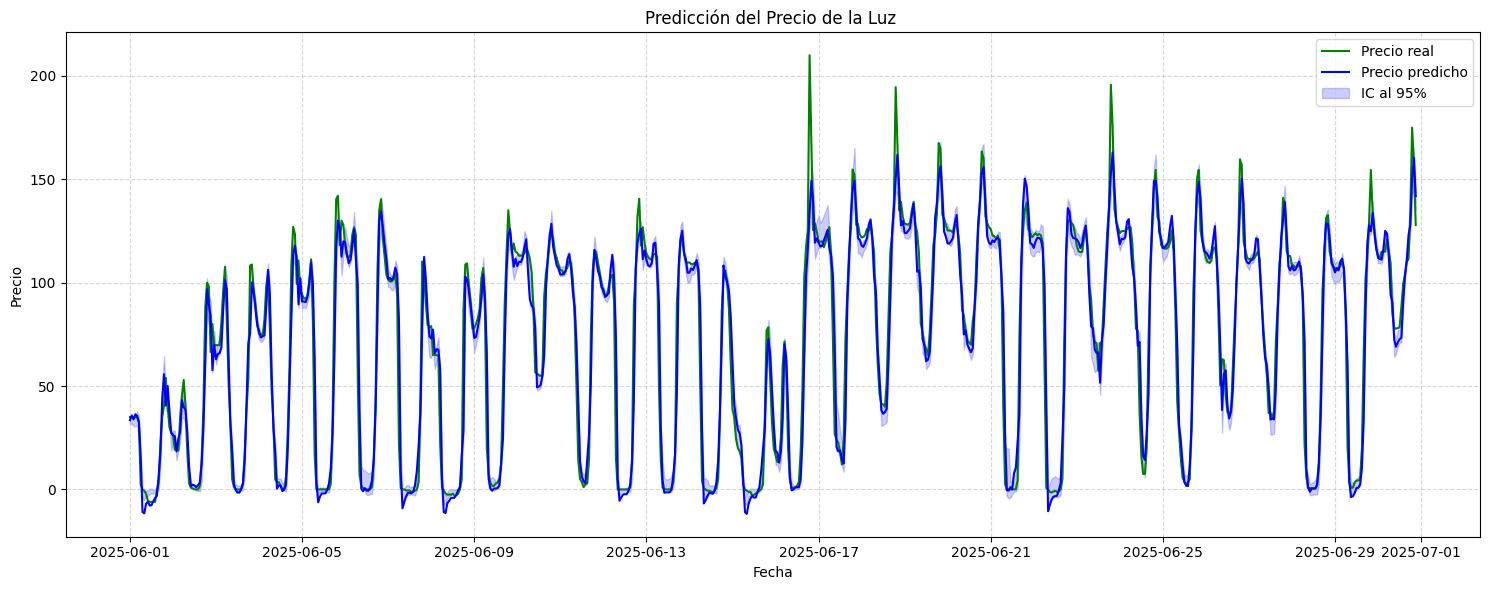
\includegraphics[width=0.7\linewidth]{figuras/XGBoost_prediccion.png}
    \caption[Predicción con XGBoost]{Se observa una predicción realizada para el mes de junio de 2025 con un entrenamiento del histórico de datos completos.}
    \label{XGBoost_prediccion}
\end{figure}
\begin{figure}[H]
    \centering
    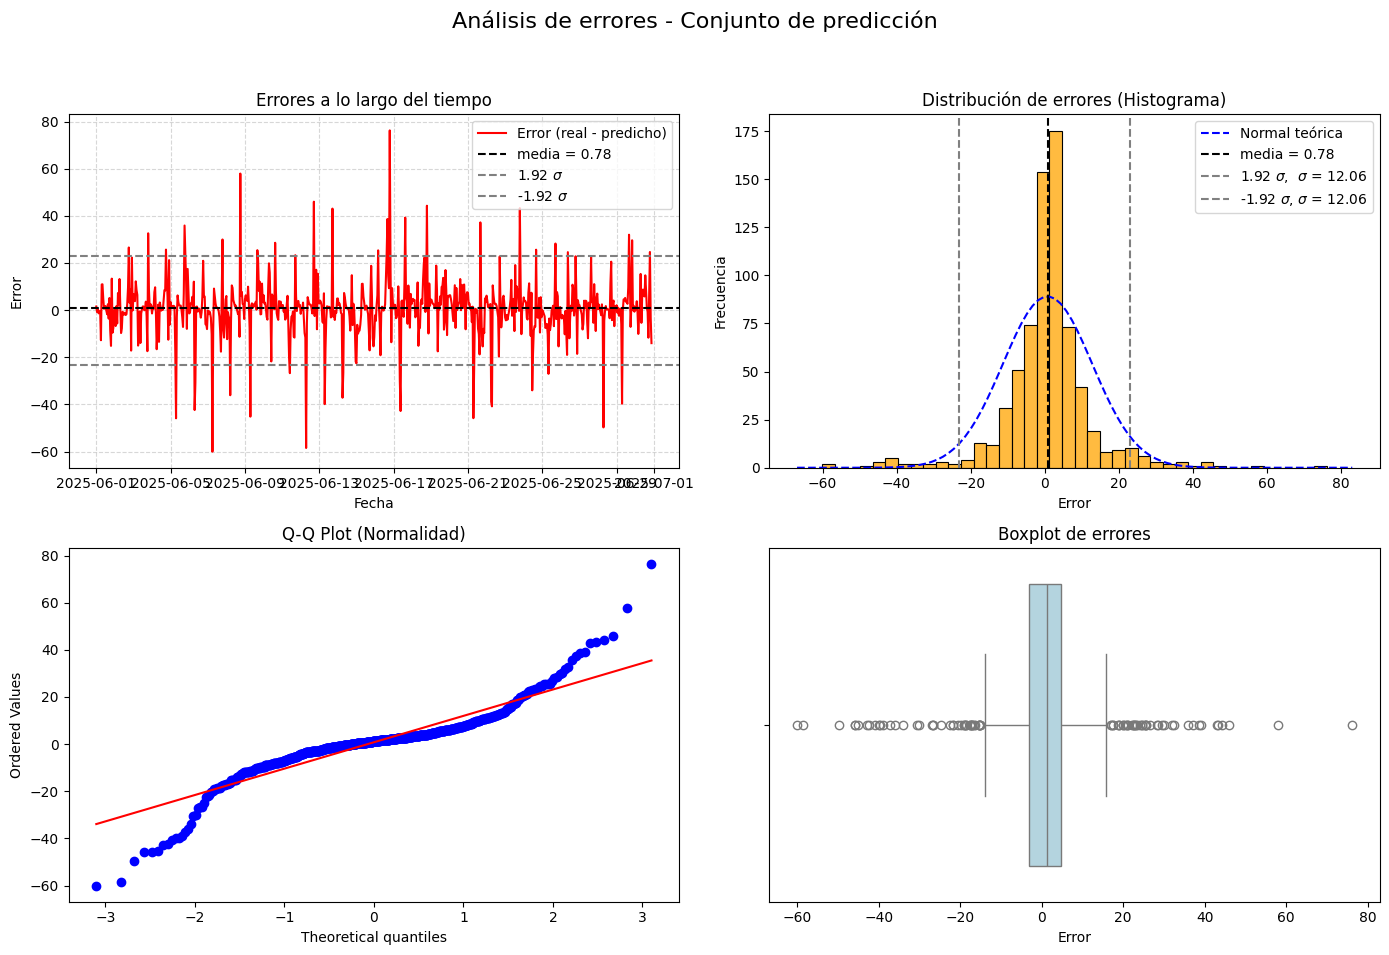
\includegraphics[width=0.7\linewidth]{figuras/XGBoost_errores.png}
    \caption[Errores en predicción con XGBoost]{Errores del modelo XGBoost, en el que destacan los QQ-plots y el histograma para caracterizar el comportamiento de los mismos. Puede verse en ellos que se distribuyen de forma simétrica, sin colas pesadas aunque no completamente normal.}
    \label{XGBoost_errores}
\end{figure}
%
%
%
\subsubsection{TFT}
\label{TFT}
%
%
%
El Temporal Fusion Transformer (TFT) es una arquitectura de deep learning diseñada específicamente para el forecasting de series temporales multi-horizonte. Combina mecanismos de atención (propios de los Transformers) con redes neuronales recurrentes y capas de gating. Sus características clave son:

\begin{itemize}
    
    \item \textbf{Manejo de Múltiples Tipos de Variables:} Integra de forma nativa variables estáticas, entradas conocidas en el futuro y variables observadas en el pasado (ej. precio, demanda).
    \item \textbf{Aprendizaje de Patrones a Múltiples Escalas:} Puede identificar patrones temporales tanto a corto como a largo plazo simultáneamente.
\end{itemize}
%
%
%
El entrenamiento consiste en:
%
%
%
\begin{itemize}
    \item \textbf{Preparación de los Datos:} Los datos se estructuran en "ventanas" de entrada de una longitud fija para predecir una "ventana" de salida (ej. las próximas 24 horas).
    \item \textbf{Ajuste del Modelo:} Se entrena una única red neuronal que aprende las interacciones entre todas las variables a lo largo del tiempo.
\end{itemize}
%
%
%
La predicción con TFT se realiza en un solo paso:
%
%
%
\begin{itemize}
    \item \textbf{Reentrenamiento:} Se ajusta el modelo final con todos los datos históricos disponibles.
    \item \textbf{Predicción Multi-Horizonte Directa:} Para generar la predicción, se le proporciona al modelo la última ventana de datos históricos disponibles. En una única pasada hacia adelante (forward pass), el modelo genera directamente todas las predicciones para el horizonte completo.
\end{itemize}
%
%
%
\begin{figure}[H]
    \centering
    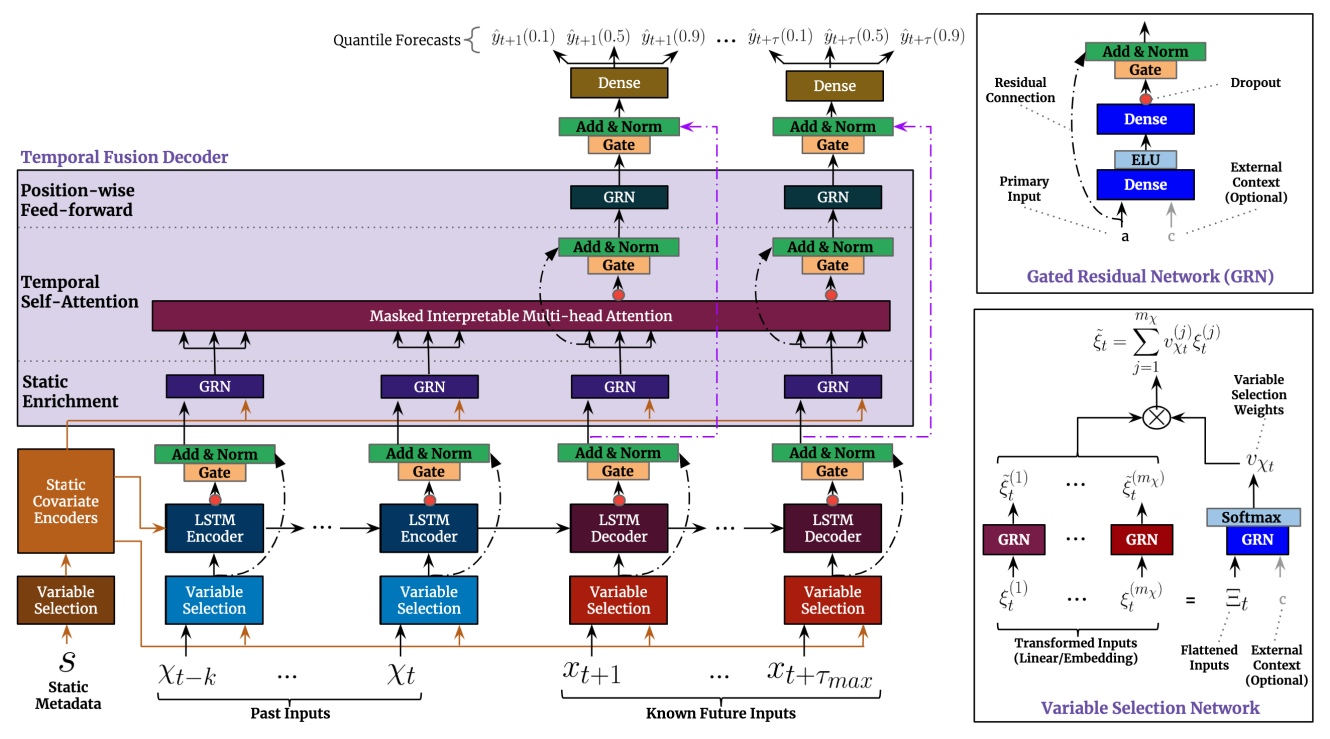
\includegraphics[width=0.7\linewidth]{figuras/TFTarquitectura.png}
    \caption[Arquitectura de TFT]{Arquitectura del TFT \cite{TFT}.}
    \label{fig:placeholder}
\end{figure}
%
%
%
Respecto a la decisión de hiperparámetros de nuestro modelo TFT es más complicada. Este tipo de modelos son más exigentes en el formato de entrada de los datos y más sensible a las configuraciones, si bien lo compensa con un gran rendimiento. Por ello no me adentraré mucho en ello:
\begin{itemize}
    \item \textbf{learning rate}: Este hiperparámetro, como se ha mencionado en el XGBoost, controla el tamaño del paso en cada iteración. Valores más altos aceleran la convergencia pero puede reportar resultados peores a costa de ellos. Por otro lado, un valor extremadamente bajo hace que la convergencia sea más lenta y puede dar lugar a que en el proceso de optimización de la función de pérdida encuentre un mínimo local y no obtenga el resultado óptimo.
    
    \item \textbf{input chunk length}: Define el número de pasos de tiempo pasados que el modelo utiliza como entrada para hacer una predicción. En nuestro caso, gicimos uso de tres mese de datos, es decir, $24 \times 7 \times 4 \times 3$ pasos de tiempo.
    \item \textbf{output chunk length}: Determina el número de pasos de tiempo futuros que el modelo debe predecir. Como se mencionó anteriormente, la predicción se realió para un mes, lo que significa $24 \times 7 \times 4$ pasos.
     
    \item \textbf{hidden size}: Se refiere a la dimensión de las capas ocultas que forman la red. En este caso, un valor demasiado alto puede elevar la complejidad del modelo, llevando a \textit{overfitting}.
     
    \item \textbf{attention heads}: Definde el número de capas de atención del modelo, es decir, nos permite regular la \textit{atención} que el TFT va a prestar a los diferentes componentes de la serie temporal de manera simultánea. Este hiperparámetro es clave para capturar las relación a largo plazo en nuestra serie.
     
    \item \textbf{dropout}: Para este tipo de modelos, un valor entre 0.1-0.3 suele ser lo estándard. Este hiperparámetro es fundamental para la regularización, previniendo el \textit{overfitting}. Consiste en desactivar aleatoriamente un porcentaje de neuronas durante el entrenamiento.
\end{itemize}

En nuestro caso particular, muestro a continuación parte del código utilizado en el que se ve cómo se refina la configuración:
\begin{lstlisting}[caption={Código de implementación del modelo TFT.}, label = {TFT_model_implementacion}]
study = optimize_hyperparameters(
    train_dataloader=train_dataloader,
    val_dataloader=val_dataloader,
    model_path="optuna_tft", 
    n_trials=500,
    max_epochs=100,
    gradient_clip_val_range=(0.01, 1.0),
    hidden_size_range=(4, 128),
    hidden_continuous_size_range=(4, 64),
    attention_head_size_range=(1, 4),
    learning_rate_range=(0.001, 0.3),
    dropout_range=(0.1, 0.3),
    trainer_kwargs=dict(
        accelerator="gpu",
        devices=1
    ),
    use_learning_rate_finder=False,
    verbose=True
)

with open("tft_study_results.pkl", "wb") as fout:
    pickle.dump(study, fout)

best_params = study.best_trial.params
print("<------------ MEJORES HIPERPARÁMETROS ENCONTRADOS ------------>")
print(best_params)

early_stop_callback = EarlyStopping(monitor="val_loss", min_delta=1e-4, patience=10, verbose=False, mode="min")
lr_monitor = LearningRateMonitor()
checkpoint_callback = ModelCheckpoint(
    dirpath="checkpoints_tft_CONbusqueda", # Cambiar carpeta cuando ejecutemos la búsqueda
    filename="tft-epoch{epoch:02d}-val_loss{val_loss:.2f}",
    auto_insert_metric_name=False,
    monitor="val_loss",
    mode="min",        
    save_top_k=1,      
    save_last=True     
)

trainer = Trainer(
    max_epochs=50,
    accelerator="gpu",
    devices=1,
    gradient_clip_val=0.1,
    callbacks=[lr_monitor, early_stop_callback, checkpoint_callback],
)

tft = TemporalFusionTransformer.from_dataset(
    training_dataset,
    learning_rate=best_params['learning_rate'],
    hidden_size=best_params['hidden_size'],
    attention_head_size=best_params['attention_head_size'],
    dropout=best_params['dropout'],
    hidden_continuous_size=best_params['hidden_continuous_size'],
    output_size=7,
    loss=QuantileLoss(),
)
print(f"Número de parámetros del modelo: {tft.size() / 1e3:.1f}k")
\end{lstlisting} 
%
%
%
\subsubsection{Resultados}
%
%
%
Para la elección de lo que podemos entender como \textit{mejor modelo} se han comparado tres métricas: MAE, RMSE y R$^2$. Una vez entreneados los modelos sobre el conjunto de entrenamiento se realiza la prueba sobre el \textit{test set} y posteriormente validamos los resultados sobre otro conjunto, del que conocemos ya los valores reales, es decir, entrenamos nuestro modelo para conocer como predice sobre los datos que le hemos introducido y después probamos sobre un conjunto, a priori de variables desconocidas, comprobando así si hemos conseguido generalizar bien el comportamiento de de la serie temporal. En la tabla siguiente se muestran los valores mencionados:
\begin{table}[H]
    \centering
    \begin{tabular}{l|ccc|ccc}
        & \multicolumn{3}{c}{Test set} & \multicolumn{3}{c}{Predicción} \\
        Modelo & MAE & RMSE & R$^2$ & MAE & RMSE & R$^2$ \\
        \hline
        SARIMAX(2,1,1)x(1,1,1,24) & 47.26 & 61.64 & -4.93 & 54.68 & 66.83 & -1.07 \\
        SARIMAX(1,1,1)x(1,1,1,24) & 47.11 & 61.77 & -4.96 & 55.00 & 67.16 & -1.09 \\
        SARIMAX(2,1,0)x(1,1,0,24) & 47.29 & 61.90 & -4.98 & 55.25 & 67.53 & -1.11 \\
        XGBoost 70/30 + RM precio  & 7.30  & 11.08 & 0.96 & 7.43  & 12.23 & 0.94 \\
        XGBoost 90/10 + RM precio  & 6.33  & 10.78 & 0.92 & 6.75  & 11.14 & 0.95 \\
        XGBoost 90/10 + RM todo    & 7.67  & 11.60 & 0.95 & 7.74  & 12.94 & 0.94 \\
        RF (SIN búsqueda) & 5.17  & 8.63  & 0.92 & 6.75  & 11.71 & 0.94 \\
        RF (CON búsqueda) & 10.09 & 14.38 & 0.76 & 13.36 & 18.64 & 0.87 \\
        TFT (SIN búsqueda)& 15.16    & 21.10    & 0.34   & 45.63    & 56.12          & -0.19 \\
        TFT (CON búsqueda NO completa)&19.43    & 24.10    & 0.52   & 25.87    & 30.19          & 0.45   \\
    \end{tabular}
    \caption{Resultados por modelos para cada conjunto de datos.}
    \label{tab:resultados_modelos}
\end{table}

A la vista de los resultados de la tabla \ref{tab:resultados_modelos} podemos observar que el modelo \textit{SARIMAX} es el que peores métricas muestra, no consiguiendo captar de manera general el comportamiento de la serie temporal. Cabe destacar en este punto que también se trata del modelo que al que menos tiempo he invertido ya que era consciente que los otros iban a reportar mejores resultados de manera más sencilla y rápida. Por otro lado, los resultados de los modelos \textit{XGBoost} y \textit{RandomForest} son parejos y muestran un buen rendimiento, siendo el \textit{XGBoost} ligeramente mejor.

En último lugar, para el TFT no he llegado a conocer los resultados finales. La implementación de la búsqueda de hiperparámetros la realicé, tal y como se ha mostrado en el \Cref{TFT}, pero debido al gran tiempo que requiere no pude realizar el análisis de este modelo. Sin embargo, este es un modelo más complejo. Se trata de una adaptación de los \textit{Transformers} (modelos de deep learning utilizados en el procesamiento de lenguaje natural como GPT) a series temporales, por lo que de él se esperan unos mejores resultados, comparables a los del \textit{XGBoost}.

\begin{figure}[H]
\centering
\begin{subfigure}[b]{0.7\textwidth}
\centering
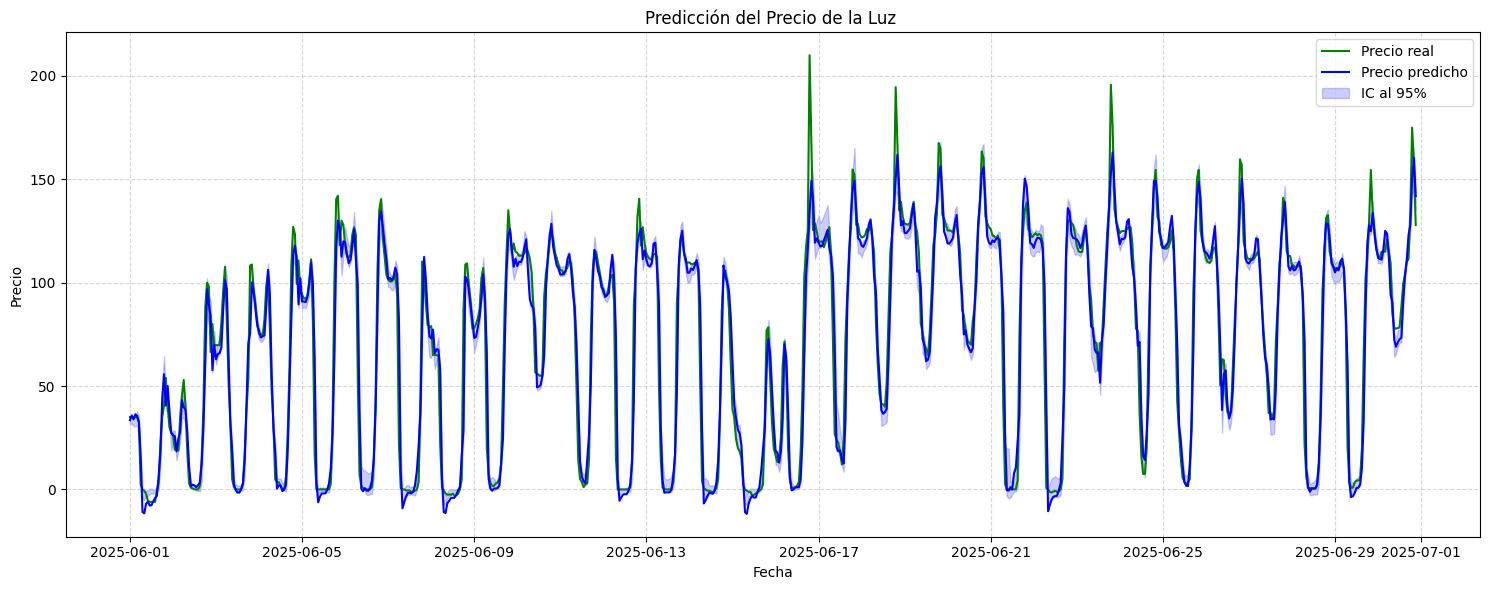
\includegraphics[width=\textwidth]{figuras/XGBoost_prediccion.png}
\caption[Resultados \textit{XGBoost}]{Resultados para el modelo \textit{XGBoost}.}
\label{ResultadosXGBoost}
\end{subfigure}
\begin{subfigure}[b]{0.7\textwidth}
\centering
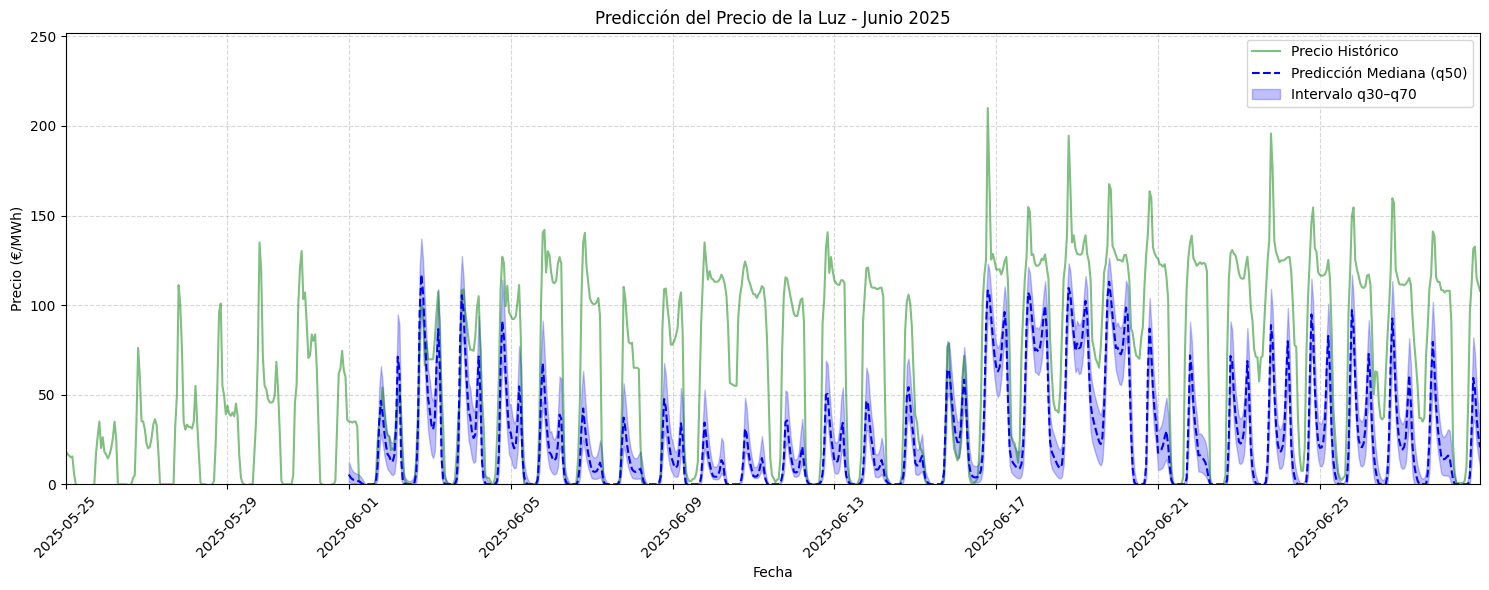
\includegraphics[width=\textwidth]{figuras/TFT_predCon1.png}
\caption[Resultados preliminares TFT.]{Resultados preliminares TFT, sin búsqueda exaustiva de hiperparámetros.}
\label{ResultadosTFT}
\end{subfigure}
\end{figure}



En conclusión, mi recomendación y sensación, dentro del contexto del proyecto, es que el modelo \textit{XGBoost} es la mejor elección en la relación de tiempo y resultados. El interés principal recaía en el comportamiento y la elección del instante en el que llevar a cabo las fundiciones y no tanto un precio muy exacto. Por lo tanto, el modelo \textit{XGBoost} es el que mejor se adapta a las necesidades del proyecto, siendo capaz de predecir con una precisión aceptable y con un tiempo de entrenamiento razonable.
%
%
%
\subsection{Modelo físico}
%
%
Con el fin de explicar con algo de detalle cómo se modela un proceso de este tipo, voy a dar una introducción teórica del proceso, para traducirlo después a términos matemáticos. Como es comprensible, no se hicieron todos estos cálculos y las suposiciones y situaciones de la práctica no requieren tanto tecnicismo. Por esto, en la parte final de esta sección explicaré brevemente qué es lo que podría resultar útil de este planteamiento de cara a su implementación para una empresa.
%
%
%
\subsubsection{Situación simplificada: Primera aproximación} \label{PrimeraAproximacion}
%
%
%
Dado un metal conocido (X) de temperatura de fusión $T_f$, calor específico en los estados sólido y líquido, $c_{\text{sol}}$ y $c_{\text{liq}}$ respectivamente, entonces a la hora de conocer cuánta energía será necesaria tendremos que tener en cuenta:
\begin{itemize}
    \item[I] El metal X a una temperatura inicial $T_0$ debe ser calentado hasta la temperatura de fusión $T_f$, esto dependerá del \textit{calor específico} del material en el estado \textit{sólido}, que viene a ser el \textit{coste} energético para aumentar la temperatura del mismo.
    \item[II] Una vez alcanzado dicho objetivo el material cambia de estado de la materia requiriendo una nueva cantidad de calor dependiente del \textit{calor latente} del material, denominado como $L_{\text{s-l}}$.
    \item[III] Finalmente supondremos que seguiremos elevando la temperatura por lo que, de manera análoga al paso I, tendremos que tener en cuenta esta energía. Llamaremos a este límite $T_c$
\end{itemize}
Para realizar dichos cálculos, haremos uso de las fórmulas de calor para calor específico y transiciones de fase.
\begin{align}
    Q_{\text{pf}} &= m \cdot c_{\text{sol}} \cdot (T_f-T_0).\\
    Q_{\text{f}} &= m \cdot L.\\
    Q_{\text{e}} &= m \cdot c_{\text{liq}} \cdot (T_c-T_f).
\end{align}
De este modo, $Q = Q_{\text{pf}} + Q_{\text{f}} + Q_{\text{e}}$. Finalmente, deberíamos tener en cuenta que los hornos no son ideales y tenemos una cierta pérdida de energía. Este hecho, cuantificado por el rendimiento $\eta \in [0,1]$, provoca un aumento en el calor total necesario: $Q^{\text{tot}} = Q/\eta$.

\subsubsection{Situación general} \label{SituacionGeneral}
%
%
%
Nos situamos ahora ante el problema general, en el que partimos de temperaturas iniciales cercanas a la ambiente ($T_0 \simeq 25 \C$) mientras que llegamos a una temperatura final, $T_f$. En este caso tendremos que aplicar la formulación general:
\begin{equation}
    Q = m \cdot \int_{T_a}^{T_b} c(T)dT,
    \label{calor}
\end{equation}
donde $m$ es la masa del compuesto X y $c(T)$ es la función del calor específico con la temperatura. Para poder operar con esta expresión sería necesario consultar datos tabulados sobre el material y una vez obtenidos los datos de $c$ para distintas temperaturas, interpolamos para obtener una función con la que calcular, de manera aproximada, el calor en la \Cref{calor}.
De este modo llegaríamos a una situación similar a la descrita en la \Cref{PrimeraAproximacion}, obteniendo $Q^{\text{tot}}$. En ambos casos, como se va a tener desarrollo polinómico de $c(T)$, podemos calcular
\begin{align}
    Q & = m \cdot \int_{T_a}^{T_b} c(T)dT = m \cdot \int_{T_a}^{T_b} \Big[a_0+ a_1 T + \dots + a_nT^n \Big]dT = \\
    & = m \cdot \Big[a_0T+ \frac{a_1}{2} T^2 + \dots + \frac{a_n}{n+1} T^{n+1}\Big] \bigg|_{T_a}^{T_b} = m \cdot p(T_a, T_b),
\end{align}
donde sustituyendo obtenemos el valor deseado. Para el primer caso, tenemos que $T_a$ coincide con la temperatura \textit{ambiente} de la pieza mientras que $T_b$ con la de fusión del material X. Por otro lado, para la etapa final, la temperatura de fusión coincide con la inicial y la final que habíamos denominado $T_f$.
\subsubsection{Traducción matemática}
La situación anterior debe ser convenientemente planteada como restricciones, de cara a la resolución del problema de optimización con el que nos encontramos. Aunando lo descrito en la \Cref{SituacionGeneral} podemos escribir que el calor $Q$ necesario para la pieza X es:
\begin{equation}
    Q = Q_{\text{pf}} + Q_{\text{f}} + Q_{\text{e}} + Q' = m \cdot \Big( p_I + L + p_{III} \Big) + Q',
\end{equation}

Finalmente, debería considerarse el rendimiento $\eta$ del horno. Podríamos suponer que este valor es aproximadamente constante de manera que $\min{\eta f(x)} = \eta \min{f(x)}$, pudiendo prescindir de este valor. Si no fuera así deberíamos formularlo como una función e introducirlo en nuestro problema con sus correspondientes restricciones. Ya por último, se ha obtenido el calor $Q$ con unidad (J) \textit{julios}, mientras que habitualmente el coste eléctrico se da en \euro/kWh por lo que deberemos realizar la debida conversión. Esta, al igual que pasa con el rendimiento, influye en el valor numérico final pero no en el problema a optimizar.
%
%
\subsubsection{Implementación}
%
%
Como se ha mencionado, el trasfondo teórico de un proceso como este es, en muchos casos, innecesario para dar una solución en el ámbito profesional, si bien es lo técnicamente correcto \footnote{Evidentemente, para llevarlo al grado más óptimo habría que introducir pérdidas de calor, más factores disipativos que puedan afectar al proceso, etc.}. Sin embargo, entender este planteamiento es importante debido a que la solución que se le otorga a una empresa está fundamenteada en ello.

Por lo general, no solo en este proyecto, sino también en la investigación realizada, lo más demandando en procesos de este tipo son las \textit{curvas de potencia} o respecto de otras magnitudes como el calor, temperatura... Del modelo planteado anteriormente podemos extraer ciertas conclusiones.

Es habitual que las empresas no tengan acceso a un histórico muy detallado del proceso, por lo que en ocasiones contamos con medidas escasas, sin embargo, podemos observar como la potencia ($P = Q/t$) crece de manera proporcional al calentamiento y depende directamente de la masa y las propiedades térmicas del material. Por ejemplo, una curva de potencia típica muestra cómo varía la demanda energética a lo largo del ciclo de fundición: inicialmente, la potencia requerida es mayor durante el calentamiento rápido, disminuyendo una vez alcanzada la temperatura de fusión y estabilizándose durante el mantenimiento térmico (una etapa muy común en fundiciones por ejemplo para eliminar impurezas).

De igual modo, las curvas de temperatura permiten visualizar el perfil térmico de la pieza, identificando los puntos críticos del proceso (como el paso por la temperatura de fusión). Estas curvas son útiles para ajustar los hiperparámetros del horno, optimizar los tiempos de ciclo y prever posibles incidencias.
%
%
\subsection{Optimización de la superficie de enfriamiento}
%
%
En último lugar, nos encontramos con el problema que aborda la distribución de las piezas metálicas obtenidas de la colada en una superficie para que enfríen. Cláramente, el objetivo es maximizar la cantidad de piezas depositadas en la misma de manera simultánea. Además de las condiciones lógicas de tamaño, se cuenta con otras restricciones como son que las piezas no son apilables (de ahí que se trate de un problema de superficie y no de volumen) y es necesario dejar unos márgenes de seguridad entre piezas. En la resolución de este problema participé en la propuesta de resolución pero no he llegado a implementar completamente ésta por lo que voy a detallar el flujo de trabajo. De manera anterior a este proceso se supone que se ha relizado la predicción de los precios de la luz y con ello una propuesta de planificación, de manera que ahora sería el momento de comprobar cómo se va a distribuir en la nave.
\subsubsection{Tamaño de cajas}
     En función del diámetro de las piezas fundidas se asignan cajas, de forma cuadrada o rectangular, rellenas de arena en las que la pieza reposará hasta la siguiente fase del proceso
\subsubsection{Chequeo de espacio} Una vez definidas las cajas, se comprueba si el área disponible es suficiente para albergar la carga de trabajo suficiente.
\begin{itemize}
    \item En caso negativo se rechaza la propuesta, mostrando datos como la superficie necesaria y ciertas combinaciones de piezas que permitirían depositar el material, por si el cliente quisiera aceptar la contrapropuesta y modificar la planificación.
    \item En caso positivo, se procede a la siguiente fase.
   \end{itemize}
Hay que remarcar aquí que, como se ha mencionado anteriormente, entre las cajas debe existir un margen de seguridad. Para incluir esto en el modelo se implementa en la función del área de cada pieza, es decir, si llamamos $A$ al área de la superficie de trabajo necesaria, de manera que $A = \sum A_i$ donde $i \in \{\text{piezas}\}$, entonces para cada pieza tendríamos que tener en cuenta que $A_i = (a+\frac{d}{2})\cdot(b+\frac{d}{2})$, con $a,b$ los lados de la caja y $d$ el margen de seguridad.
\subsubsection{Distribución de superficie} 
Una vez validada la propuesta, se procede a distribuir las cajas. Para ello se tienen que tener en cuenta la forma de la superficie, dado que hay que diferenciar entre la capacidad de almacenaje y la capacidad de distribución, me explico: Podríamos tener una superficie rectangular con una gran número de cajas que dividan mi área en dos zonas, por ejemplo de $2$ m$^2$, entonces no podríamos introducir una pieza de $4$ m$^2$ aunque quisiéramos. Matemáticamente hablando deberíamos ver cómo de conexa es nuestra superficie.

Una vez superada esta parte, se procede a distribuir las piezas, colocando las más grandes en primer lugar y se van comprobando de manera combinatoria las posibilidades del resto. Esta forma de actuar, a fuerza bruta, se eligió porque ciertamente no se contaba con un gran número de piezas por lo que la complejidad de un problema como este, que crece como $n!$ si $n$ es el número de piezas, no sería un gran problema en la práctica. Si contasemos con un mayor número de cajas se debería optar por un algoritmo mucho más refinado que disminuyera la cantidad de prueba-error.

\subsubsection{Ejemplo de implementación}

Como se ha mencionado, no he llegado a implementar completamente este proceso, sin embargo, si realicé una pequeña parte de la implementación, que se muestra a continuación. En este caso, se trata de un ejemplo sencillo en el que se comprueba si una superficie rectangular es capaz de albergar una serie de cajas con unas dimensiones concretas y un margen de seguridad.

\begin{figure}[H]
    \centering
    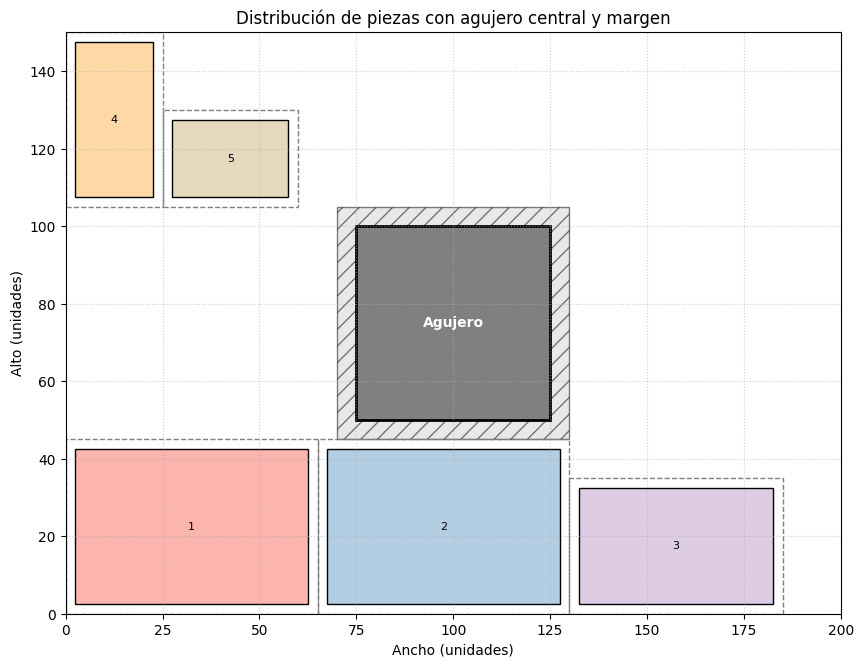
\includegraphics[width=0.6\linewidth]{figuras/ejemplo_packaging.png}
    \caption[Ejemplo distribución de superficie]{Ejemplo de la distribución de las cajas en la superficie de enfriamiento. Para ello se hizo uso de la librería \textit{rectpack}, que permite realizar el problema de la mochila en 2D, o el \textit{bin packing} con rectángulos (y por tanto cuadrados).}
    \label{fig:ejemplopackaging}
\end{figure}
%
\begin{lstlisting}[caption={Código de implementación del problema de distribución de piezas.}, label={distribucion_piezas}]
    packer = newPacker(pack_algo=GuillotineBafSas, rotation=True)
for rect in pieces_sorted:
    packer.add_rect(*rect)
for w, h in sub_bins:
    if w > 0 and h > 0:
        packer.add_bin(w, h)
packer.pack()
fig, ax = plt.subplots(figsize=(10, 8))
colors = plt.cm.get_cmap('Pastel1', len(pieces))
coordenadas_finales = []
ax.add_patch(plt.Rectangle((hx, hy), hw, hh, facecolor='lightgray', edgecolor='black', lw=1, alpha=0.5, hatch='//'))
ax.add_patch(plt.Rectangle((hole_x, hole_y), hole_w, hole_h, facecolor='gray', edgecolor='black', lw=2))
ax.text(hole_x + hole_w/2, hole_y + hole_h/2, "Agujero", ha='center', va='center', color='white', weight='bold')
piece_idx = 0
for bin_idx, abin in enumerate(packer):
    bin_x, bin_y = sub_bin_positions[bin_idx]
    for rect in abin:
        x_margin, y_margin, w_margin, h_margin = rect.x + bin_x, rect.y + bin_y, rect.width, rect.height
        piece_w = w_margin - margin
        piece_h = h_margin - margin
        piece_x = x_margin + margin / 2
        piece_y = y_margin + margin / 2
        coordenadas_finales.append({
            "pieza": piece_idx + 1, "x": piece_x, "y": piece_y,
            "ancho": piece_w, "alto": piece_h
        })
        ax.add_patch(plt.Rectangle((x_margin, y_margin), w_margin, h_margin,
                                     facecolor='none', edgecolor='gray', lw=1, linestyle='--'))
        ax.add_patch(plt.Rectangle((piece_x, piece_y), piece_w, piece_h,
                                     facecolor=colors(piece_idx), edgecolor='black', lw=1))
        ax.text(piece_x + piece_w/2, piece_y + piece_h/2, f'{piece_idx+1}', 
                ha='center', va='center', fontsize=8, color='black')
        
        piece_idx += 1
ax.set_xlim(0, container_width)
ax.set_ylim(0, container_height)
ax.set_aspect('equal', adjustable='box')
ax.set_title("Distribución de piezas con agujero central y margen")
plt.xlabel("Ancho (unidades)")
plt.ylabel("Alto (unidades)")
plt.grid(True, linestyle=':', alpha=0.6)
\end{lstlisting}
%
%
